\subsection{Parameter Estimation Results}
The one step ahead prediction results for CFTP test data is presented bellow. CFTP data has the most noise and $u_2$ is zero for the first 600 seconds of the test resulting in PE condition not being satisfied for the first half of the data. This can be seen in the plot of the maximum eigen value which remains at the initial value for the same duration and then quickly converges to zero when non-zero $u_2$ data is available. The prediction error is higher than expected and further analysis of the governing equations is required for improving the model.
\begin{figure}[H]
        \centering
        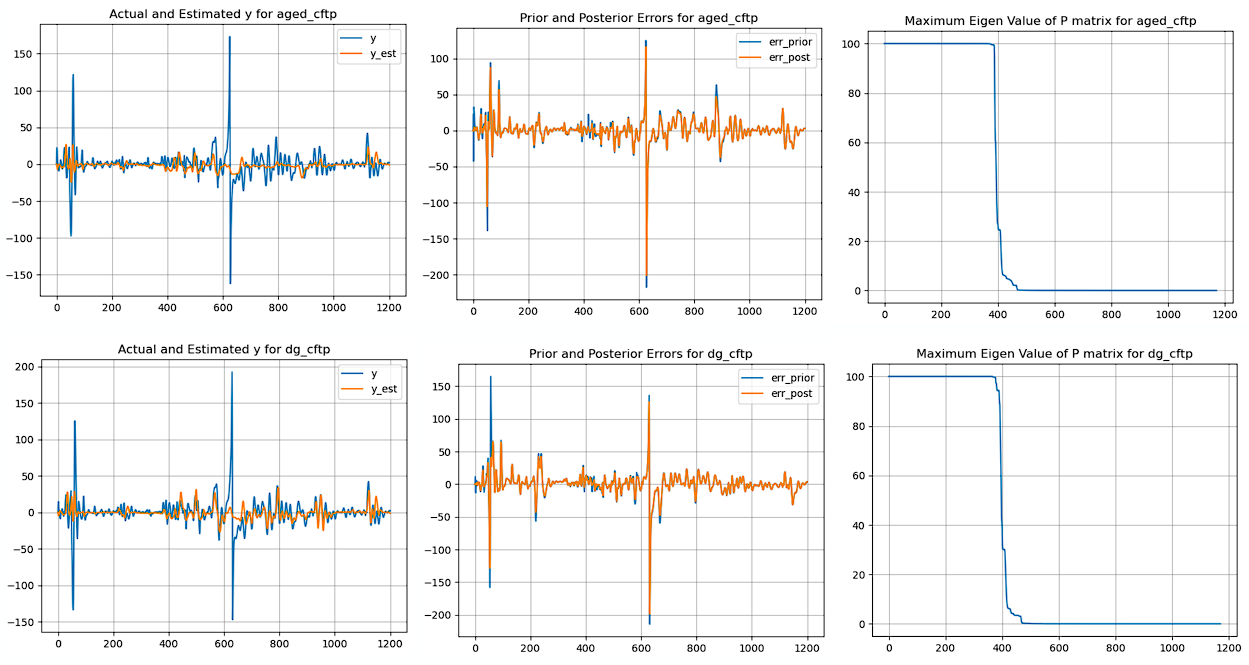
\includegraphics[width = \textwidth]{\froot/figs/par_est_results/RLS_results_cftp.png}
        \caption{1-step prediction, error priors and posteriors, and the maximum eigen value of the covariance matrix in RLS}
\end{figure}
The parameter estimates from least-squares is presented bellow. The estimation is done both by using individual data sets and combining the data of the tests from $600 s$ to $900 s$ based on the aging level. These 8 estimates (3 for each of the test and 1 for mixed data, for each aging level) are plotted to see if the parameter vectors cluster based on the aging level.
\begin{figure}[H]
        \centering
        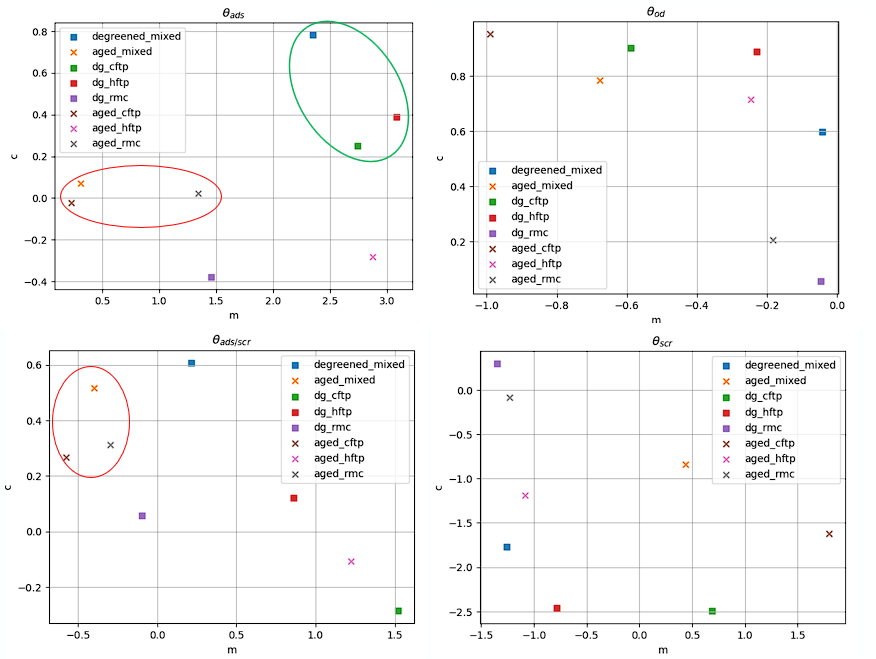
\includegraphics[width = 0.75\textwidth]{\froot/figs/par_est_results/par_estimates.png}
        \caption{Parameter estimates from the test-cell data}
\end{figure}
More data is need to show the statistical significance of the clustering of the parameter vectors based on the aging level.
